\chapter{Algoritmo de Búsqueda}

\section{Flujo y funcionamiento}

El algoritmo de busqueda es el descrito en el RFC 1034~\cite{RFC1034} sección 4.3.2, el cual se encarga recibir la consulta DNS y responder acorde a esta, buscando los registros en la base de datos del servidor.
Este algoritmo contempla distintos escenarios, desde lo más general hasta lo más específico. Un resumen del mismo es el siguiente:

\begin{itemize}
    \item Primero, se verifica si el dominio consultado pertenece al catálogo del servidor.  
    Si no pertenece, se responde con el código \texttt{REFUSED}, indicando que el servidor no es autoritativo para dicho dominio.
    \begin{itemize}
        \item Si el dominio consultado y el tipo de registro solicitado existen en la base de datos, se responde directamente con los registros encontrados.
        \item Si el tipo de registro solicitado no es \texttt{CNAME}, pero existe un registro \texttt{CNAME} para el dominio, se realiza una nueva llamada a la función de búsqueda utilizando el valor del \texttt{CNAME} como nuevo nombre de dominio y conservando el tipo original.  
        Los registros \texttt{CNAME} encontrados se agregan a la respuesta final.
    \end{itemize}

    \item Si el proceso anterior no produce una respuesta, se continúa con la búsqueda de \texttt{glue records} y \texttt{wildcards}:
    \begin{itemize}
        \item Si el dominio posee un \texttt{glue record} en la base de datos, se responde con dicho registro.
        \item En caso contrario, se verifica si existe un \texttt{wildcard} aplicable al dominio consultado.
        \begin{itemize}
            \item Si se encuentra un \texttt{wildcard}, se responde con los registros asociados a él.
            \item Si no se encuentra ningún \texttt{wildcard}, se responde con \texttt{NXDOMAIN}, indicando que el dominio no existe.
        \end{itemize}
    \end{itemize}
\end{itemize}

Este proceso está simplificado, la versión de código es bastante más compleja y además cubre el estandar de DNSSEC. A contiuación se mostrará un diagrama de flujo de la función \texttt{lookup\_data}, 
la cual es la función principal. Luego en otras subsecciones se explicará en detalle las funciones auxiliares.

\begin{figure}[h!]
    \centering
    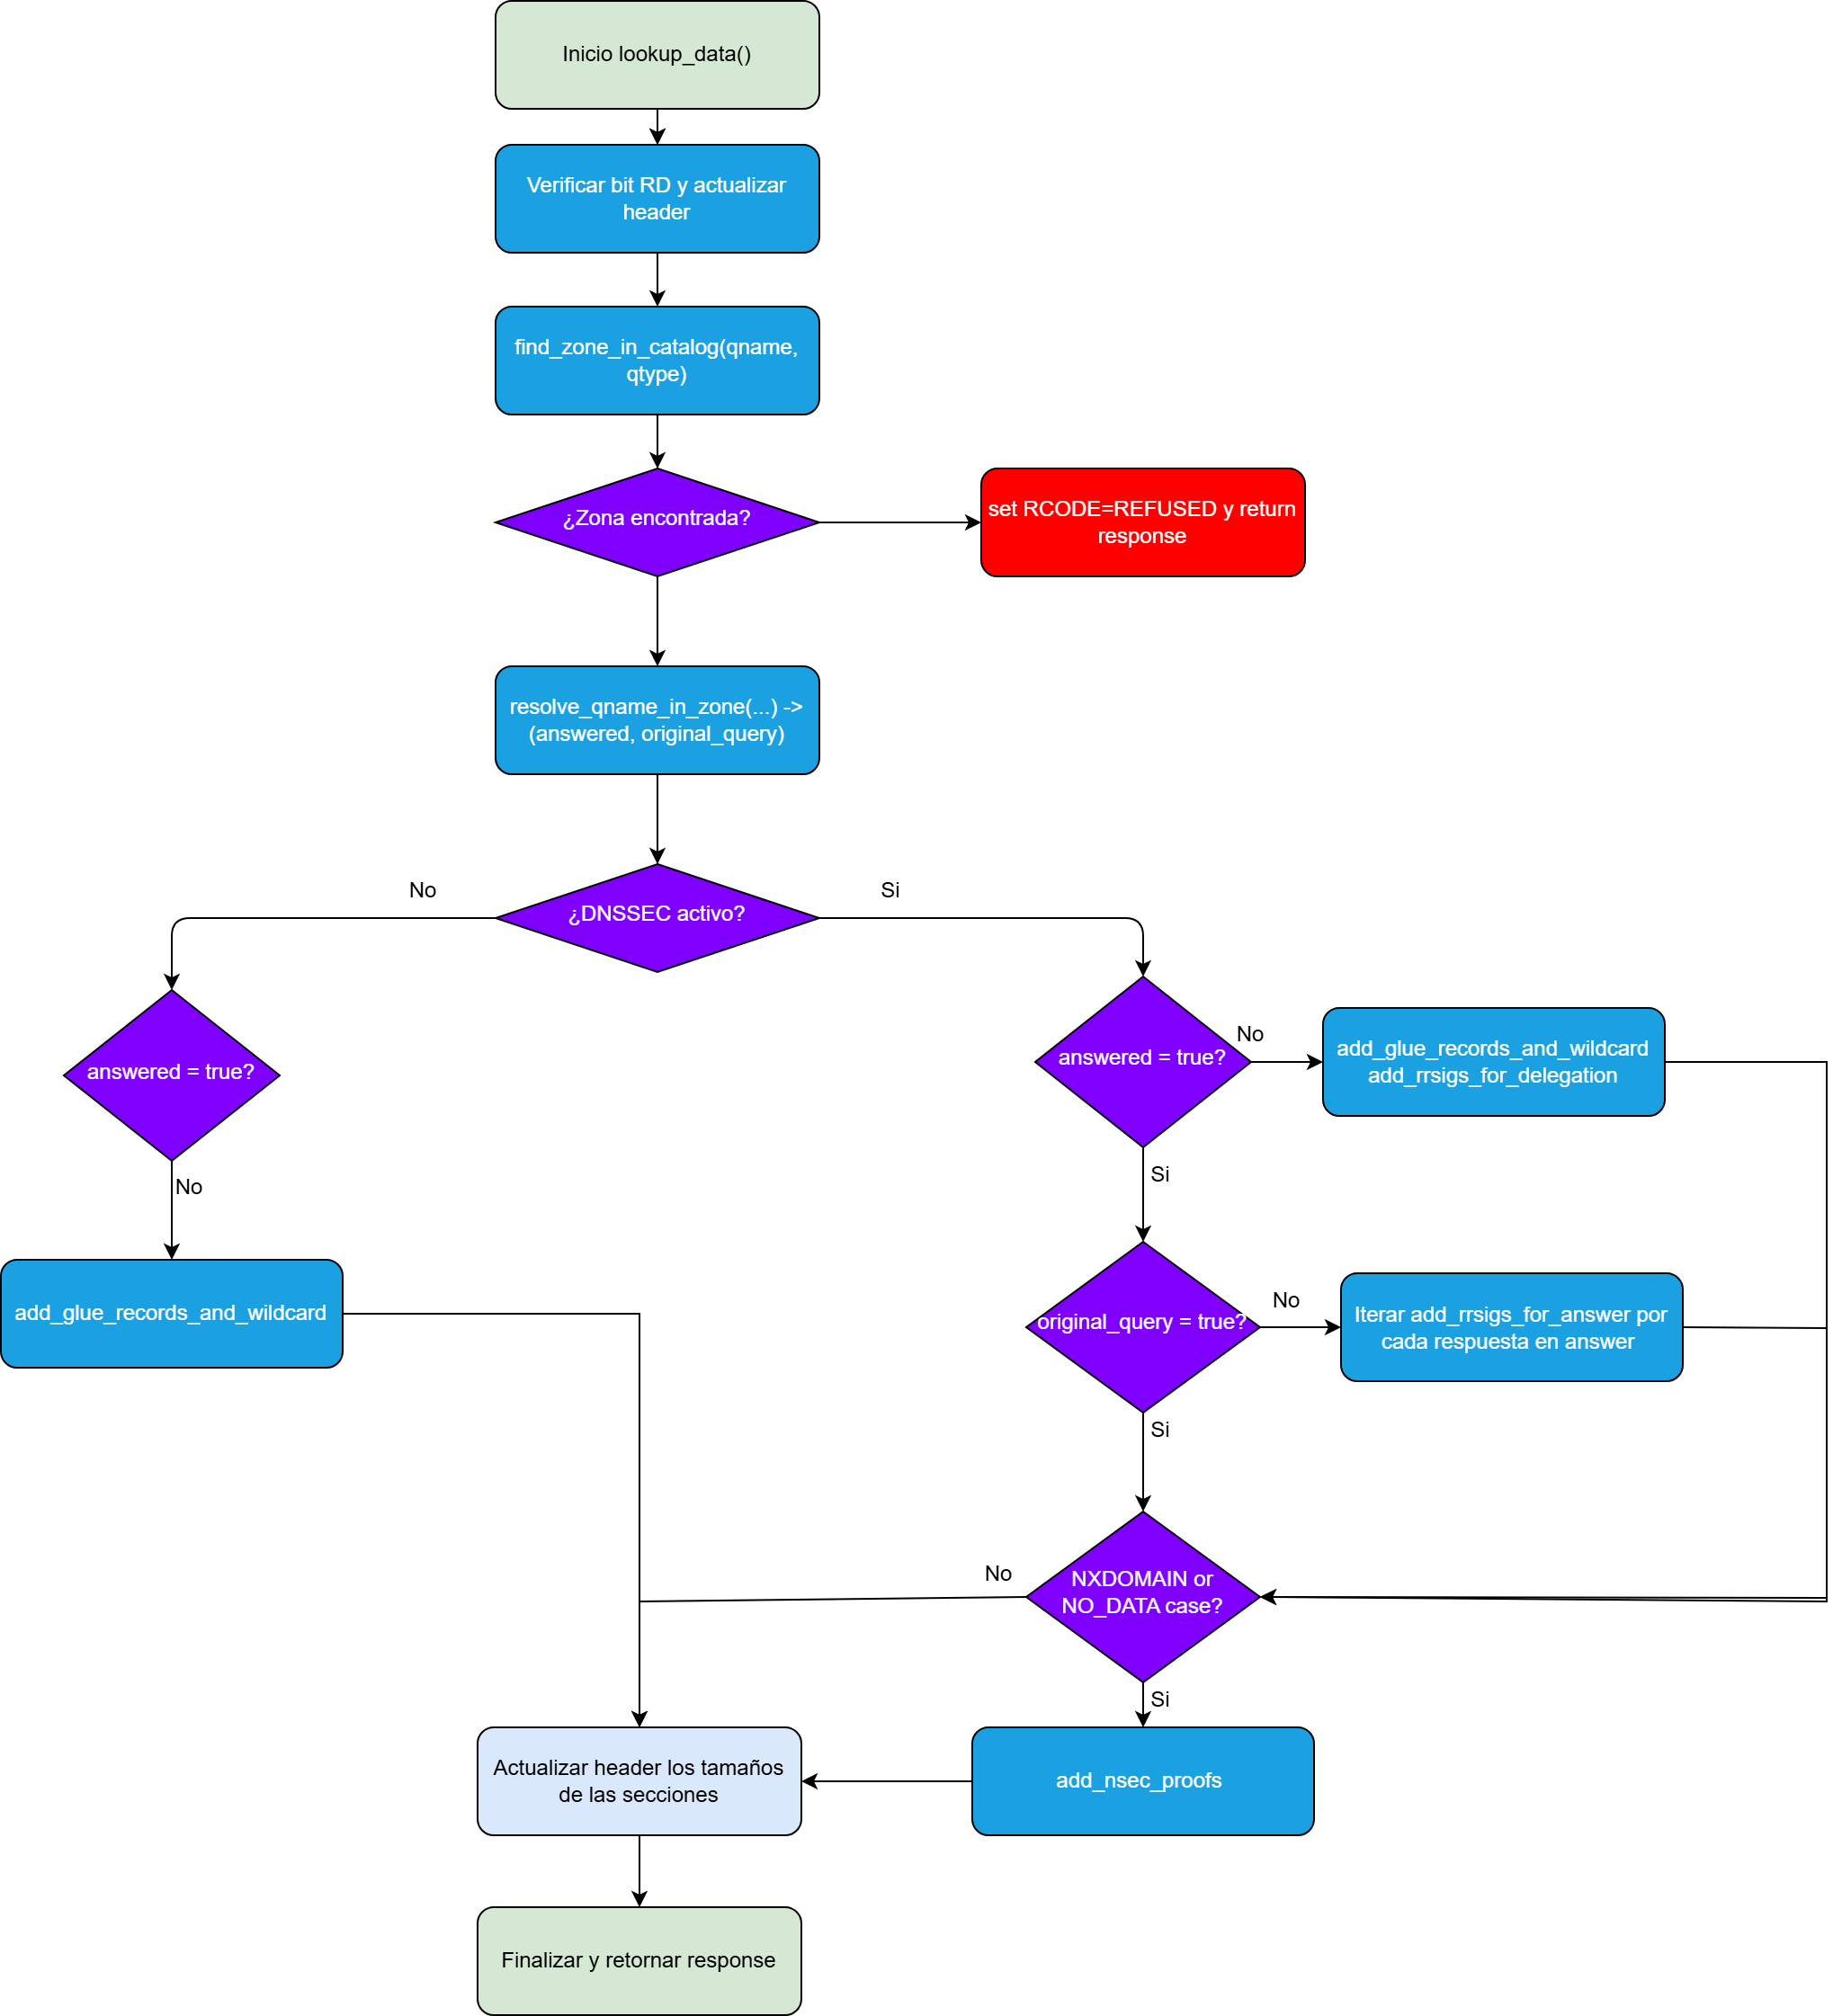
\includegraphics[width=1.1\textwidth]{diagramas/lookup_data.png}
    \label{fig:lookup_data_flowchart}
\end{figure}

La función \texttt{lookup\_data} recibe como parámetros la consulta DNS completa y la bandera que indica si el modo DNSSEC está activado. A partir de la consulta, 
se extraen el nombre de dominio y el tipo de registro solicitado, y se inicia el proceso de búsqueda.

Primero, la función intenta localizar la zona correspondiente en el catálogo. Si la zona existe, se procede a resolver el nombre mediante la función \texttt{resolve\_qname\_in\_zone},
la cual realiza la resolución directa o a través de registros internos. Esta función retorna dos valores booleanos:


\begin{itemize}
    \item answered: Indica si la consulta fue respondida correctamente.
    \item \texttt{original\_query}: Verdadero cuando la respuesta incluye registros del tipo solicitado originalmente, y falso cuando la respuesta se basa en un \texttt{CNAME} intermedio.
\end{itemize}

Si la consulta se realiza con \texttt{DNSSEC} habilitado, se añaden los registros de firma \texttt{RRSIG} correspondientes a los registros presentes en la respuesta. 
En caso de que no se haya podido responder, se agregan los \texttt{glue records}, posibles \texttt{wildcards} y sus respectivas firmas \texttt{RRSIG}.
Cuando la respuesta no corresponde a la consulta original (es decir, proviene de \texttt{CNAMEs}), se añaden también las firmas \texttt{RRSIG} de dichos registros adicionales. 
Además, si la respuesta corresponde a un error \texttt{NXDOMAIN} o a un caso \texttt{NO\_DATA}, se incluyen los registros \texttt{NSEC} que sirven como prueba criptográfica de inexistencia.

Por otro lado, si \texttt{DNSSEC} no está activo, el proceso se simplifica: si no se obtuvo una respuesta directa, se intenta completar la información añadiendo \texttt{glue records} o 
\texttt{wildcards}.

Finalmente, se actualizan los contadores y tamaños de las secciones en el encabezado (\texttt{HEADER}), y la función retorna la respuesta completa.

A continuación se explican cada una de las funciones auxiliares que componen el algoritmo de búsqueda.

\subsection{find\_zone\_in\_catalog}

Esta función recibe el nombre de dominio consultado y el tipo de registro y busca por cada subdomoinio del domino original si existe una zona en el catálogo que maneje ese dominio.
Por ejemplo si el dominio consultado es \texttt{a.niclabs.cl}, la función buscará en el catálogo las zonas \texttt{a.niclabs.cl}, \texttt{niclabs.cl}, \texttt{cl} y \texttt{root}. 
Si encuentra una zona que maneje alguno de estos dominios, retorna la estructura de datos de la zona vista en la sección~\ref{main-sec:catalogo}.

Esta función es bastante simple pero maneja casos especiales que son importantes y que vienen desde el estandar de DNSSEC. Por ejemplo si tipo consultado es \texttt{DS},
la función debe retornar la zona padre, ya que los registros DS son manejados siempre por la zona padre. Además existe un problema con el nombre de dominio raíz, ya que como se verá
en una sección posterior, el nombre de dominio raíz se maneja internamente como \texttt{root} ya que no se puede usar \texttt{"."} como nombre de carpeta en el sistema de archivos. Por lo tanto, si 
el dominio consultado es \texttt{"."} la función debe buscar la zona \texttt{root} en el catálogo.

\subsection{resolve\_qname\_in\_zone} 

Esta función traduce en lógica programática el paso 3.a del algoritmo definido en el RFC 1034~\cite{RFC1034}, gestionando de forma coherente la búsqueda interna, 
la detección de alias, las delegaciones y los casos sin datos dentro de una zona DNS.

Se puede dividir el funcionamiento de esta función en los siguientes pasos:

\subsubsection{Presencia de un registro CNAME}

Si el nombre consultado posee un registro CNAME, la función distingue dos situaciones:

\begin{itemize}
    \item Si el tipo solicitado \textbf{NO} es \texttt{CNAME}, el registro \texttt{CNAME} se añade igualmente a la respuesta, ya que informa que el nombre consultado es un alias. A continuación, 
          el algoritmo sustituye el nombre original por el destino del \texttt{CNAME} y reinicia la búsqueda con ese nuevo nombre.
    \item Si el tipo solicitado es \texttt{CNAME}, se agregan los registros \texttt{CNAME} encontrados a la respuesta y se considera la consulta resuelta. 
\end{itemize}

En ambos casos, el bit de respuesta autoritativa (AA) se marca como verdadero, indicando que la información proviene directamente de la zona local.

\subsubsection{Coincidencia exacta con nombre y tipo solicitado (distinto a CNAME)}

Si el nombre posee registros del tipo consultado, estos se incorporan a la sección de respuestas. En este punto, la función evalúa si los registros corresponden a servidores de nombres (\texttt{NS}). 
Si el conjunto \texttt{NS} pertenece al apex de la zona (al nombre de la zona, por ejemplo \texttt{niclabs.cl}), la respuesta es autoritativa; si pertenece a un subdominio delegado, la función interpreta
que se trata de una delegación y desactiva el bit de autoridad. De este modo, el comportamiento refleja la distinción entre datos autoritativos y delegaciones establecida por el RFC.

\subsubsection{El nombre existe, pero no hay datos del tipo solicitado (\texttt{NO\_DATA})}
Cuando el nombre se encuentra en la zona pero no existen registros del tipo pedido, la función retorna con un código de respuesta NOERROR, indicando que el nombre es válido 
pero no posee información del tipo solicitado. Este caso corresponde al escenario “no data”, en el cual no se genera un error, sino simplemente una respuesta vacía.

\subsubsection{El nombre no existe en la zona}

Si el nombre de dominio no aparece en los datos de la zona, el algoritmo finaliza sin agregar información a la respuesta. La ausencia total de datos para ese nombre
será tratada posteriormente por otra función que añade wildcards y/o NSECs segun corresponda. Hasta este punto el codigo de respuesta debería ser \texttt{NXDOMAIN} pero
no se asigna aún, ya que podría cambiar si se encuentran \texttt{wildcards} o \texttt{glue records}.

El diagrama de flujo de esta función es el siguiente:

\begin{figure}[h!]
    \centering
    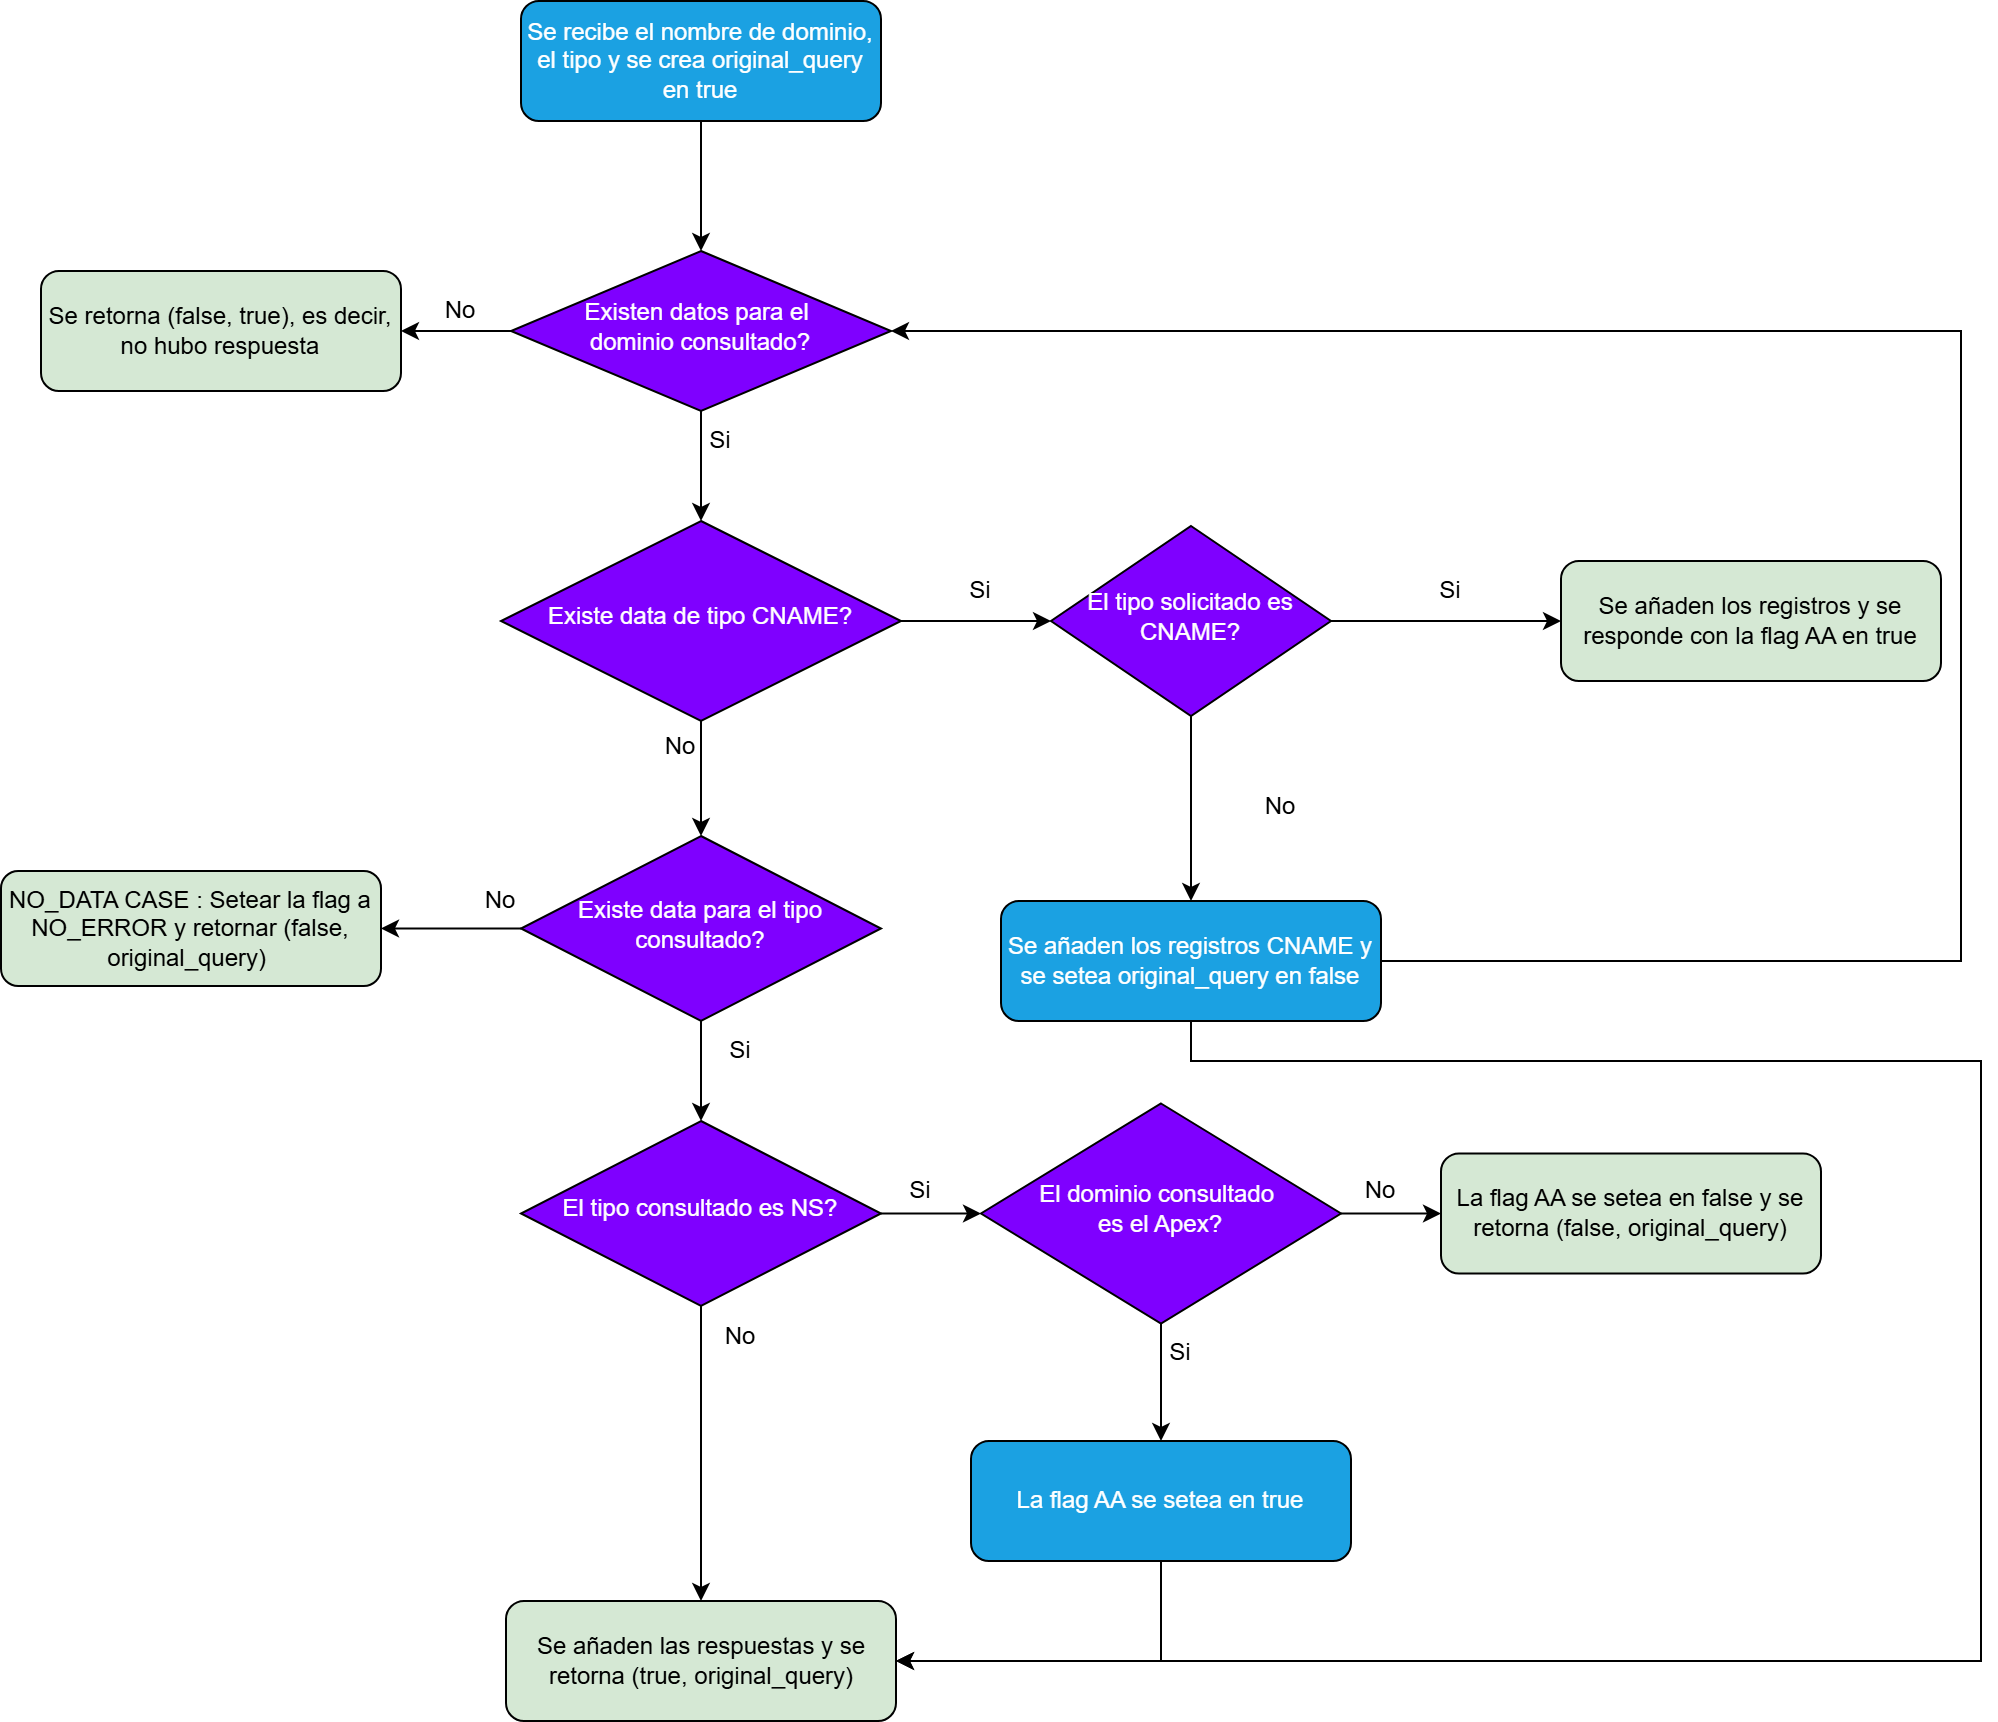
\includegraphics[width=1.1\textwidth]{diagramas/resolve_qname_in_zone.png}
    \label{fig:resolve_qname_in_zone_flowchart}
\end{figure}


\subsection{add\_glue\_records\_and\_wildcard}

La función \texttt{add\_glue\_records\_and\_wildcard} implementa las secciones 3.b y 3.c del algoritmo de búsqueda. Su objetivo principal es manejar los 
casos de \texttt{delegations} (referrals) y de coincidencias con \texttt{wildcards}.

En primer lugar, la función analiza si el dominio consultado (\texttt{qname}) corresponde a un punto de delegación. Para ello, busca si existen registros \texttt{NS} 
asociados al nombre, y verifica que dicho conjunto de registros no esté acompañado por un \texttt{SOA}. Si existen registros \texttt{NS} sin \texttt{SOA}, significa que el 
dominio actual marca el inicio de una subzona delegada, por lo que el servidor debe responder con una \texttt{referral}. En este caso:

\begin{itemize}
    \item Todos los registros \texttt{NS} encontrados se copian en la sección \texttt{Authority} de la respuesta.
    \item Luego, por cada nombre de servidor listado en esos registros \texttt{NS}, se busca si existe un registro \texttt{A} o \texttt{AAAA} correspondiente 
          (denominado \texttt{glue record}). Si se encuentran, estos se añaden en la sección \texttt{Additional}.
\end{itemize}

Una vez construida la \texttt{referral}, el código establece el campo \texttt{Rcode} en \texttt{NOERROR} y marca la respuesta como no autoritativa (\texttt{AA = 0}), 
dado que el servidor no es responsable de la zona delegada.


Si no se encuentra un punto de delegación, el algoritmo continúa con la búsqueda de coincidencias mediante \texttt{wildcards}.
Para ello, si existe un registro \texttt{RRset} asociado al \texttt{wildcard} y que coincida con el tipo de consulta (\texttt{qtype}), entonces:

\begin{itemize}
    \item Se añaden los registros encontrados a la sección \texttt{Answer}, utilizando como nombre propietario el \texttt{qname} original (según lo especificado por el RFC, aunque la firma se haya generado sobre el \texttt{wildcard}).
    \item Si existen firmas digitales \texttt{RRSIG} que cubran el tipo solicitado, estas si corresponde se añaden igualmente en la sección \texttt{Answer}.
    \item Además, se incluyen en la sección \texttt{Authority} los registros \texttt{NSEC} y sus firmas \texttt{RRSIG} asociadas, cuando corresponda.
\end{itemize}

Finalmente, si no se encuentra ningún \texttt{wildcard} aplicable:
\begin{itemize}
    \item Si la consulta actual corresponde al nombre original, el servidor determina si se trata de un caso \texttt{NO\_DATA} (nombre existente sin registros del tipo solicitado). 
          En tal caso, responde con \texttt{NOERROR} y \texttt{AA = 1}.
    \item En caso contrario, responde con \texttt{NXDOMAIN} (nombre inexistente) y también marca la respuesta como autoritativa.
\end{itemize}
 
Aclarar que \textbf{NO} se añaden los \texttt{RRSIG} en los glue record ya que la respuesta \textbf{NO} es autoritativa en ese caso.

\newpage


El diagrama de flujo de la función descrita es el siguiente:

\begin{figure}[h!]
    \centering
    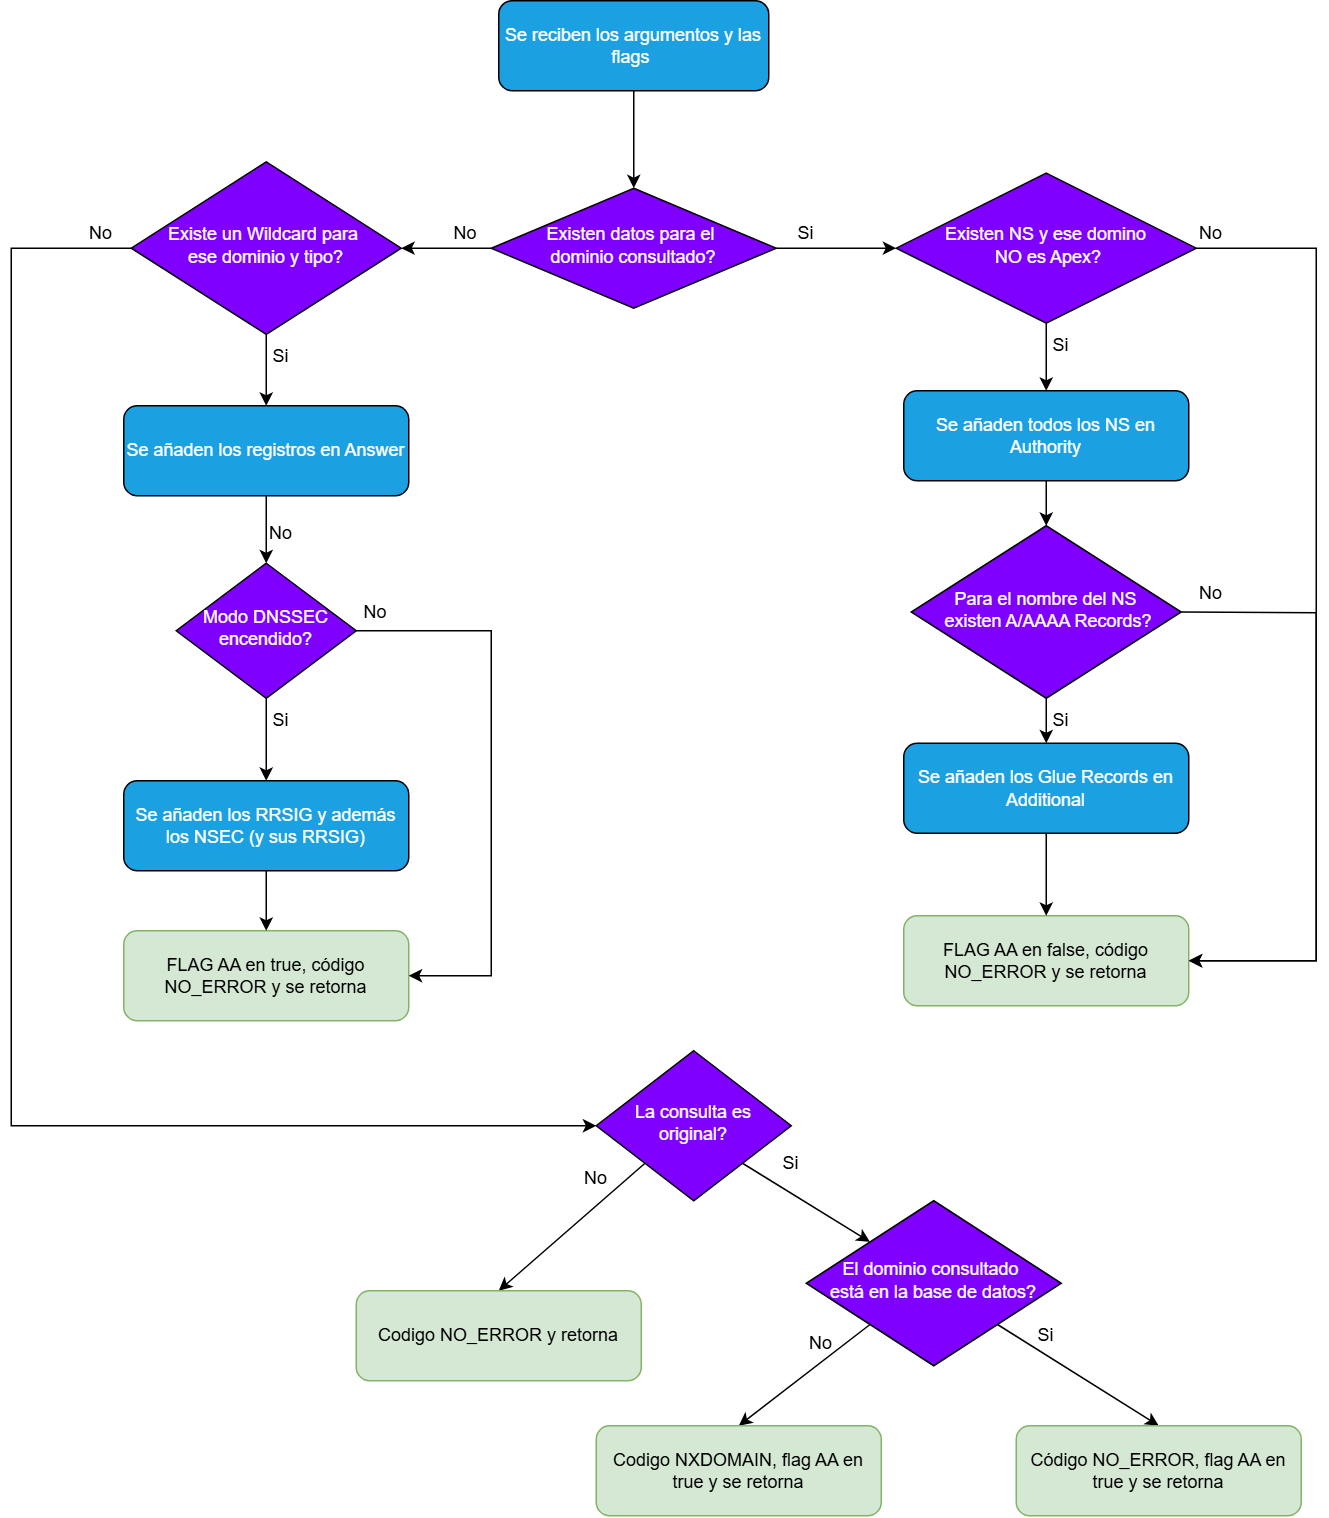
\includegraphics[width=1.1\textwidth]{diagramas/add_glue_records_and_wildcard.png}
    \label{fig:add_glue_records_and_wildcard_flowchart}
\end{figure}



\subsection{\texttt{add\_rrsigs\_for\_delegation}}

Esta función se encarga de añadir los registros \texttt{DS} y sus correspondientes firmas \texttt{RRSIG} a la sección de autoridad del mensaje DNS (\texttt{response}) cuando se 
genera una respuesta de delegación en un servidor DNSSEC.

En términos simples, cuando el servidor responde indicando que un dominio está delegado (por ejemplo, cuando responde con un conjunto de registros \texttt{NS} que apuntan al 
servidor autoritativo de una subzona), esta función busca si en su base de datos también existen los registros \texttt{DS} y sus firmas digitales (\texttt{RRSIG}) correspondientes, y 
los incluye en la respuesta.

El envío de los registros \texttt{DS} junto con una delegación está descrito en el RFC 4035, sección 2.3 (“Response Generation: Including DS and NSEC Records”).
Aclarar también que esta función se ejecuta siempre independientemente de si la hubo o no un referral, ya que si no hay \texttt{DS}  simplemente se omite su adición. Este aspecto podría
ser mejorado en el futuro para evitar llamadas innecesarias a la función.


\subsection{add\_rrsigs\_for\_answer}

Esta función se encarga de añadir los registros \texttt{RRSIG} correspondientes a un conjunto de registros de respuesta en la sección \texttt{Answer} del mensaje DNS (\texttt{response}).

En el contexto de DNSSEC, cada conjunto de registros (\texttt{RRset}) debe estar acompañado por su firma digital
(\texttt{RRSIG}), que permite a los resolvers validar criptográficamente que los datos no han sido alterados.

La función solo añade los RRSIG correspondiente al tipo de consulta original, es decir, si la consulta fue por registros \texttt{A}, 
solo se añadirán los \texttt{RRSIG} que firman los registros \texttt{A}. 

El comportamiento descrito está definido en el RFC 4035, sección 2.2 (“Response Generation: Including RRSIG Records”).

\newpage

\subsection{add\_nsecs\_proofs}

Esta función se encarga de añadir las pruebas criptográficas de inexistencia (\texttt{NSEC} y \texttt{RRSIG(NSEC)})
a la sección Authority del mensaje DNS (\texttt{response}) cuando el servidor genera una respuesta
de tipo \texttt{NODATA} o \texttt{NXDOMAIN} bajo DNSSEC.

Para dar contexto, los registros \texttt{NSEC} son registros especiales en DNSSEC que indican qué nombres de dominio y tipos de registros existen dentro de una zona firmada.
Para hacer esto, cada registro \texttt{NSEC} enlaza un nombre de dominio con el siguiente en orden canónico, y contiene un mapa de bits que indica qué tipos de registros están presentes para ese dominio.
Un orden canonico es un orden lexicográfico de los nombres en minúsculas.

Por ejemplo , si se tiene un registro \texttt{NSEC} que indica que el dominio \texttt{example.com} tiene registros \texttt{A} y \texttt{MX}, y enlaza con \texttt{foo.example.com},
esto significa que \texttt{example.com} existe y tiene esos tipos de registros, y que el siguiente dominio en orden canónico es \texttt{foo.example.com}, por lo tanto cualquier nombre entre 
\texttt{example.com} y \texttt{foo.example.com} no existe en la base de datos.

La función maneja los siguientes dos casos principales:

\subsubsection{Caso 1: el dominio existe, pero el tipo de registro no (respuesta \texttt{NODATA})}
Si el dominio consultado está presente en la base de datos, pero no tiene registros del tipo solicitado (\texttt{qtype}),
entonces se deben incluir los registros \texttt{NSEC} y \texttt{RRSIG(NSEC)} asociados a ese mismo dominio en la sección Authority.

Estos registros demuestran que, aunque el nombre existe, no hay ningún registro del tipo solicitado (por ejemplo, no existe un \texttt{MX} para ese dominio).
Esto se hace a través del mapa de tipos de registro contenidos en el registro \texttt{NSEC}, que indica qué tipos de registros están presentes para ese dominio.


\subsubsection{Caso 2: el dominio no existe (respuesta \texttt{NXDOMAIN})}

Si el dominio consultado no está en la base de datos, se necesita saber cual registro \texttt{NSEC} cubre el rango que incluye el nombre inexistente.

Para ello, se realiza una búsqueda binaria en la lista de nombres \texttt{NSEC}:

\begin{itemize}
    \item Si el dominio es menor que todos los nombres existentes, se utiliza el último nombre de la lista (por la naturaleza circular del espacio de nombres DNSSEC).
    \item En caso contrario, se toma el nombre inmediatamente anterior al dominio consultado.
\end{itemize}

Aclarar que la comparación entre dominios se realiza en su forma canónica.

Luego, se insertan en la respuesta los registros \texttt{NSEC} y \texttt{RRSIG(NSEC)} del propietario determinado. El uso de los registros \texttt{NSEC} para demostrar la 
inexistencia de nombres o tipos de registros está definido en el RFC 4035, sección 3.1.3 (“Authenticated Denial of Existence”).

Está sería la última función explicada del algoritmo de búsqueda. Con esto se cierra el capítulo.

A continuación se mostrarán respuestas del algoritmo para distintos casos de prueba en la sección [REDACTED].

\newpage

\section{Resultados según cada caso de consulta}

A continuación se muestran ejemplos de respuestas generadas por el algoritmo de búsqueda para distintos casos de consulta. Cada ejemplo incluye los records presentes en la base de datos, 
la consulta realizada y la respuesta generada en el formato del comando \texttt{dig}.

Aclarar que la sección Additional no se añadirá en los ejemplos a menos que contenga registros, para simplificar la visualización.

\subsection{Consulta con coincidencia exacta con rtype y el nombre de dominio}

\begin{table}[h!]
\centering
\begin{tabular}{llll}
\textbf{Nombre de dominio} & \textbf{Clase} & \textbf{Tipo} & \textbf{Data} \\
\hline
\texttt{www.example.com.} & IN & A & 0.0.0.0 \\
\texttt{www.example.com.} & IN & A & 0.0.0.1 \\
\end{tabular}
\end{table}

Al preguntar directamente por la IP de \textbf{www.example.com} se encuentra una coincidencia exacta con el nombre y el tipo solicitado en los datos, por lo que la 
respuesta DNS tendrá todos los \texttt{RRs} del \texttt{RRset} en la sección \texttt{Answer}, además de los \texttt{RRSIG} correspondientes:\\

\begin{lstlisting}
;; ->>HEADER<<- opcode: QUERY, status: NOERROR, id: 4660
;; flags: qr aa; QUERY: 1, ANSWER: 3, AUTHORITY: 0, ADDITIONAL: 1

;; QUESTION SECTION:
;www.example.com.          IN      A

;; ANSWER SECTION:
www.example.com.   3600    IN      A       192.0.2.1
www.example.com.   3600    IN      A       192.0.2.2
www.example.com.   3600    IN      RRSIG   A 8 3 3600 0 0 12786 www.example.com. (keydata ...)
\end{lstlisting}

\subsection{Consulta con coincidencia solo en el nombre de dominio, pero existe un registro CNAME}

\begin{table}[h!]
\centering
\begin{tabular}{llll}
\textbf{Nombre de dominio} & \textbf{Clase} & \textbf{Tipo} & \textbf{Data} \\
\hline
\texttt{blog.example.com} & IN & CNAME & blog2.example.com. \\
\texttt{blog2.example.com.} & IN & A & 1.2.3.4 \\
\end{tabular}
\end{table}

Al consultar por \textbf{blog.example.com} el algoritmo encuentra un registro de tipo CNAME y lo guarda en la sección \texttt{Answer}. Luego, 
ejecuta nuevamente el algoritmo utilizando el nombre de dominio especificado en el CNAME, logrando así encontrar el registro con la dirección IP correspondiente.\\

\begin{lstlisting}
;; ->>HEADER<<- opcode: QUERY, status: NOERROR, id: 4660
;; flags: qr aa; QUERY: 1, ANSWER: 4, AUTHORITY: 0, ADDITIONAL: 1

;; QUESTION SECTION:
;blog.example.com.         IN      A

;; ANSWER SECTION:
blog.example.com.   3600    IN      CNAME   blog2.example.com.
blog2.example.com.  3600    IN      A       1.2.3.4
blog.example.com.   3600    IN      RRSIG   CNAME 8 3 3600 0 0 12786 blog.example.com. (keydata ...)
blog2.example.com.  3600    IN      RRSIG   A 8 3 3600 0 0 12786 blog2.example.com. (keydata ...)

\end{lstlisting}

\subsection{Consulta que sale de la zona autoritativa : Referral con Glue Records}

\begin{table}[h!]
\centering
\begin{tabular}{llll}
\textbf{Nombre de dominio} & \textbf{Clase} & \textbf{Tipo} & \textbf{Data} \\
\hline
\texttt{b.example.com} & IN & NS & ns.a.b.example.com. \\
\texttt{ns.a.b.example.com.} & IN & A & 4.3.2.1 \\
\end{tabular}
\end{table}

Al consultar por la IP de \textbf{b.example.com}, se encuentra un registro de tipo \texttt{NS}. Al comprobar que no existe ningún registro \texttt{SOA} en ese dominio 
(lo que indica que el servidor no es autoritativo en este caso), se debe guardar el registro \texttt{NS} en la sección \texttt{Authority}. Además, se debe verificar si 
existe un registro \texttt{glue} correspondiente y, de ser así, añadirlo en la sección \texttt{Additional}.\\

Además se añade el registro \texttt{DS} y su firma \texttt{RRSIG} correspondiente en la sección \texttt{Authority}, esto ya que se está delegando
a una subzona. También se añade el registro \texttt{NSEC} para confirmar la inexistencia del registro \texttt{A} solicitado a través del mapa de bits.\\

\begin{lstlisting}
;; ->>HEADER<<- opcode: QUERY, status: NOERROR, id: 4660
;; flags: qr; QUERY: 1, ANSWER: 0, AUTHORITY: 5, ADDITIONAL: 2

;; QUESTION SECTION:
;b.example.com.            IN      A

;; AUTHORITY SECTION:
b.example.com.     3600    IN      NS      ns.a.b.example.com.
b.example.com.     3600    IN      DS      12345 8 2 (digest_data ...)
b.example.com.     3600    IN      RRSIG   DS 8 3 3600 0 0 12786 b.example.com. ( keydata ... )
b.example.com.     3600    IN      NSEC    ns1.example.com. NS DS NSEC
b.example.com.     3600    IN      RRSIG   NSEC 8 3 3600 0 0 12786 example.com. ( keydata ... )

;; ADDITIONAL SECTION:
.                  32768   IN      OPT     4096
ns.a.b.example.com. 3600   IN      A       4.3.2.1
\end{lstlisting}


\subsection{Consulta sin coincidencia en el nombre de dominio pero existe un wildcard}

\begin{table}[h!]
\centering
\begin{tabular}{llll}
\textbf{Nombre de dominio} & \textbf{Clase} & \textbf{Tipo} & \textbf{Data} \\
\hline
\texttt{*.example.com.} & IN & A & 0.0.0.0 \\
\end{tabular}
\end{table}


Al consultar por cualquier dominio que no exista en los datos pero sea subdominio de \textbf{example.com}, como por ejemplo \textbf{unknown.example.com}, se 
usará el wildcard y se guardará la respuesta en la sección \texttt{Answer}. Además se añaden los registros \texttt{NSEC} y \texttt{RRSIG(NSEC)} correspondientes en la sección \texttt{Authority} para
probar la inexistencia del nombre consultado.\\

\begin{lstlisting}
;; ->>HEADER<<- opcode: QUERY, status: NOERROR, id: 4660
;; flags: qr aa; QUERY: 1, ANSWER: 2, AUTHORITY: 2, ADDITIONAL: 1

;; QUESTION SECTION:
;unknown.example.com.      IN      A

;; ANSWER SECTION:
unknown.example.com.  3600    IN      A       0.0.0.0
unknown.example.com.  3600    IN      RRSIG   A 8 2 3600 0 0 12786 example.com. ( keydata ... )

;; AUTHORITY SECTION:
*.example.com.        3600    IN      NSEC    b.example.com. A RRSIG NSEC
*.example.com.        3600    IN      RRSIG   NSEC 8 3 3600 0 0 12786 example.com. ( keydata ... )
\end{lstlisting}

\subsection{Consulta sin coincidencia en nombre de dominio y sin wildcard: NXDOMAIN}

Acá no se muestra lo que hay en la base de datos, ya que el cliente consultará por la IP de un dominio que no existe (\texttt{unknown.example.com}) y no hay wildcard que aplique. 
Para lograr esta respuesta se borró temporalmente el wildcard de los datos.\\

\begin{lstlisting}
;; ->>HEADER<<- opcode: QUERY, status: NXDOMAIN, id: 4660
;; flags: qr aa; QUERY: 1, ANSWER: 0, AUTHORITY: 2, ADDITIONAL: 1

;; QUESTION SECTION:
;unknown.example.com.      IN      A

;; AUTHORITY SECTION:
example.com.         3600    IN      NSEC    b.example.com. NS SOA RRSIG NSEC DNSKEY
example.com.         3600    IN      RRSIG   NSEC 8 2 3600 0 0 12786 example.com. ( keydata ... )
\end{lstlisting}

En la respuesta en formato DIG no se ve pero el rcode es \texttt{NXDOMAIN}.

\subsection{Consulta sin coincidencia en el tipo y sin wilcard: NODATA}

\begin{table}[h!]
\centering
\begin{tabular}{llll}
\textbf{Nombre de dominio} & \textbf{Clase} & \textbf{Tipo} & \textbf{Data} \\
\hline
\texttt{www.example.com.} & IN & A & 1.2.3.4 \\
\end{tabular}
\end{table}

Al consultar por un tipo que no existe para un dominio que sí existe, como por ejemplo pedir un registro \texttt{MX} para \textbf{www.example.com},
se responde con \texttt{NODATA} y se añaden los registros \texttt{NSEC} y \texttt{RRSIG(NSEC)} correspondientes en la sección \texttt{Authority} para
probar la inexistencia del tipo solicitado a través del mapa de tipos.\\

\begin{lstlisting}
;; ->>HEADER<<- opcode: QUERY, status: NOERROR, id: 4660
;; flags: qr aa; QUERY: 1, ANSWER: 0, AUTHORITY: 2, ADDITIONAL: 1

;; QUESTION SECTION:
;www.example.com.          IN      MX

;; AUTHORITY SECTION:
www.example.com.     3600    IN      NSEC    blog.example.com. A RRSIG NSEC
www.example.com.     3600    IN      RRSIG   NSEC 8 3 3600 0 0 12786 example.com. ( keydata ... )
\end{lstlisting}

El codigo de respuesta es \texttt{NOERROR} pero no hay registros en la sección \texttt{Answer}, siendo esto equivalente a un caso de \texttt{NO\_DATA}.
    


